\documentclass{article}

\usepackage[a4paper, total={6in, 9in}]{geometry}


\usepackage[utf8]{inputenc}
\usepackage{amsmath}
\usepackage{amsfonts}
\usepackage{amssymb}

\usepackage{amsthm}
\usepackage{french}

\usepackage{graphicx}

\usepackage{hyperref}
\hypersetup{
    colorlinks=true,
    linkcolor=blue,
    filecolor=magenta,      
    urlcolor=cyan,
}

\begin{document}

\section{La Théorie}

\subsubsection{Tableau de données}

L'Analyse en Composante Pricipale s'interesse à l'etude des tableaux de données rectangulaires dont les colonnes sont appelées \textit{Variables} et les lignes sont appelées \textit{Individus}.
\newline

L'image ci-dessous illustre un tableau de donnees a \textit{p-Variables} et a \textit{n-Individus}. Un individu est noté $X_i=(x_{i1},x_{i2}, ... ,x_{ij}, ... ,x_{ip})$ où $i=1..n$.

\begin{figure}[h!]
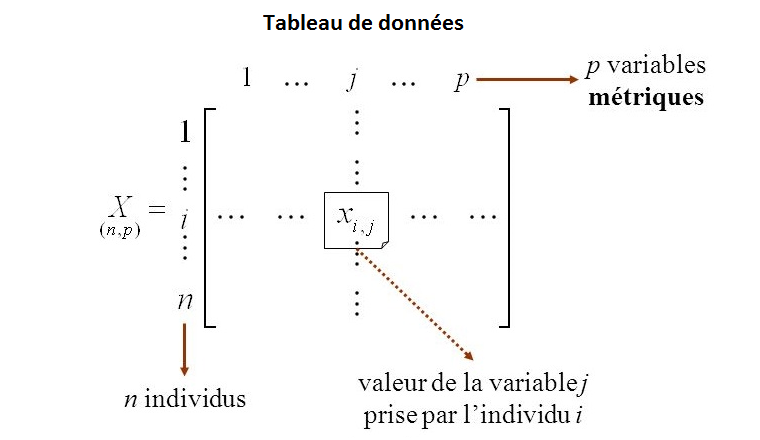
\includegraphics[width=\linewidth]{images/tableau.png}
\end{figure}

\subsubsection{Moyenne et Variance}

Pour une \textit{variable} ${x_k}$, on note sa moyenne $\bar{x_k}$ et sa variance $\sigma_k$ telles que:

\begin{equation*}
\bar{x_k}=\frac{1}{n}\sum_{i=1}^{n}{x_{ik}} \;\;\;\;\;\;\;\;\;\;\;\; \sigma_k=\frac{1}{n}\sum_{i=1}^{n}{(x_{ik}-\bar{x_{k}})^2}
\end{equation*}

\subsubsection{Distance et Centre de Gravité}

On define la distance d entre deux \textit{individus} $i$ et $j$ par:

\begin{equation*}
d^2(i,j)=\sum_{k=1}^{p}{(x_{ik}-x_{jk})^2} 
\end{equation*}




\newpage

\section{La pratique}

\subsection{Les données}

Nous allons étudier les résultats des épreuves de Decastar et des Jeux Olympiques, dont les \textit{Individus} sont les joueurs et les \textit{Variables} sont les jeux eux même, soient:
\newline
\\
- 100m, pour la course de vitesse 100m \\
- Longueur, pour le saut en longueur \\
- Poids, pour le lancé de poids \\
- Hauteur, pour le saut en hauteur \\
- 400m, pour la course de 400m \\
- 110m H, pour la course de vitesse 110m Homme \\
- Disque, pour le lancé de disque \\
- Perche, pour le lancé de perche \\
- Javelot, pour le lancé de javelot \\
- 1500m, pour la course d'endurance 1500m \\
- Classement, pour la classement finale de chaque joueur \\
- Points, pour le point finale obtenu par chaque joueur \\
- Competition, pour le type de compétition \\

Voici une partie des données utilisées:

\begin{figure}[h!]
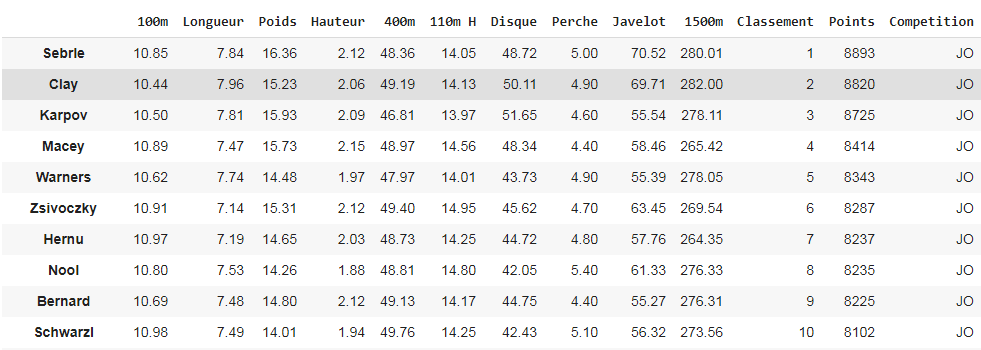
\includegraphics[width=\linewidth]{images/data_initials.png}
\end{figure}

On voit bien ici que les \textit{Variables} ne sont pas de même unité, alors on va d'abord les \underline{normalisées}. On peut confirmer que les \textit{Variables} sont bien normalisées quand elles sont asymptotiquement de moyenne nulle et de variance égale a un.

\begin{figure}[h!]
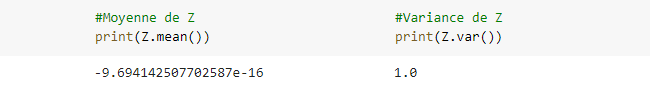
\includegraphics[width=\linewidth]{images/mean_variance.png}
\end{figure}

D'après ces résultats, les moyennes et les variances de nos \textit{Variables Normalisées} tendent bien vers 0 et 1 respectivement.
\newline

A partir d'ici, on va travailler avec les \textbf{Données Normalisées} 

\newpage

\subsection{Les variables explicatives}

Parfois, il y a des \textit{Variables} dont l'importance est néglisable par rapport aux autres, il est important de les reconnaitre ou même de les éliminer pour avoir une meilleur analyse des données. Les \textit{Variables} restantes issue de cette \underline{élimination} seront appelées \textit{Variables Explicatives}.
\newline

Il y a plusieurs méthodes pour retrouver les variables à éliminer, mais pour notre problème, on va utiliser la méthode du coudé, d'après \href{https://fr.qaz.wiki/wiki/Elbow_method_(clustering)}{Wikipedia - Méthode du coude (clustering)} 
\newline

\textit{La méthode du coude est une heuristique utilisée pour déterminer le nombre de clusters (Variables dans notre cas) dans un ensemble de données . La méthode consiste à tracer la} \textbf{variation expliquée} \textit{en fonction du nombre de clusters, et à choisir le coude de la courbe comme le nombre de clusters à utiliser. La même méthode peut être utilisée pour choisir le nombre de paramètres dans d'autres modèles basés sur les données, comme le nombre de composants principaux pour décrire un ensemble de données}
\newline

Pour ce faire, on a donc besoin des variation expliquée de chaque \textit{Variable} de notre données normalisées et de trace la courbe de la fonction f définie par:

\begin{equation*}
f(V_e)=\frac{(n-1)}{n}*V_e \quad , \; V_e \; est \; la  \; variance \; explicative.
\end{equation*}

\begin{figure}[h!]
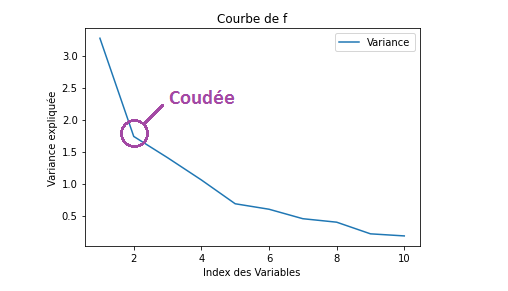
\includegraphics[width=\linewidth]{images/courbe_ve.png}
\end{figure}

D'après la graphe de la fonction - variance expliquée - on ne va donc retenir que les deux premières \textit{Variables} qui sont: la \textit{Variable 100m} et la \textit{Variables Longueur}.
\newline

\newpage

A partir de ces deux \textit{Variables}, on peut positionner les individus dans le plan. On a alors la figure suivante:

\begin{figure}[h!]
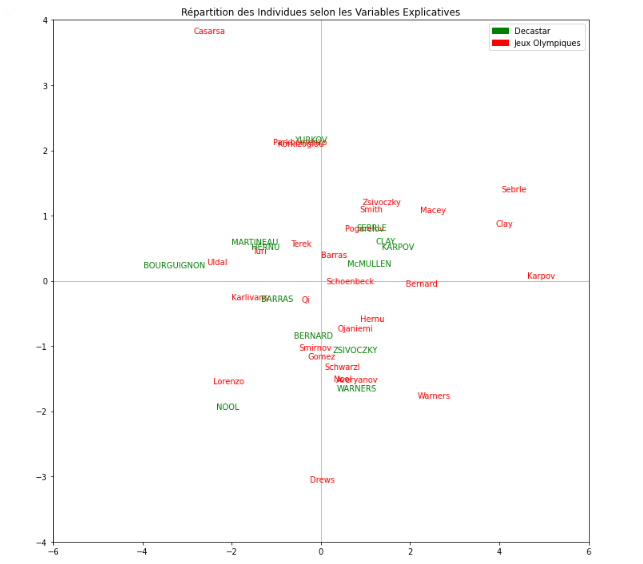
\includegraphics[width=\linewidth]{images/graph-plan.png}
\end{figure}

\subsubsection{Interpretation}

\underline{\textbf{Premier Axe}}: On peut remarquer du premier axe qu'elle departage les joueurs ayant un bon classement a ceux qui ont un mauvais classement pendant les deux competitions.
En effet, les joueurs \textbf{Karpov} et \textbf{Clay} qui sont le deuxieme et le troisieme dans le classement des Jeux Olympiques, et des Jeux de Decastar sont placés à droite dans la premier axe alors que le joueur \textbf{Uldal}, avant dernier du classement des JO et le joueur \textbf{Bourguignon}, dernier du classement de Decastar sont placés a gauche dans la premier axe. 
\newline
\underline{\textbf{Deuxieme Axe}}: On peut remarquer du deuxieme axe qu'elle departage les joueurs  

\begin{figure}[h!]
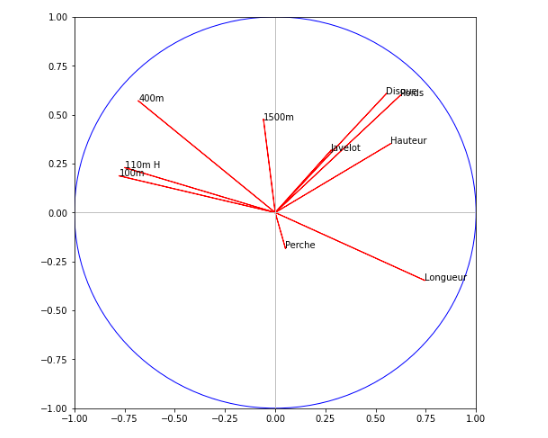
\includegraphics[width=\linewidth]{images/cercle_cor.png}
\end{figure}



\end{document}
